\documentclass{ReportTemplate}
\usepackage{titlesec}
\title{CSEL}
\author{Macherel Rémy}
\date{\today}
\subtitle{Rapports des TP}
\subsubtitle{Git du projet : \href{https://github.com/Mathistis/csel-workspace}{https://github.com/Mathistis/csel-workspace}}
\location{Fribourg,}
\contact{remy.macherel@master.hes-so.ch}
\version{1.0}
\titlespacing*{\chapter}{0pt}{-60pt}{20pt}
\begin{document}

\maketitlepage

\newpage

\maketableofcontent

\medskip

\titleformat{\chapter}[display]
    {\Huge\bfseries}
    {}
    {0pt}
    {\thechapter.\ }
    

\chapter{TP Systèmes de fichiers}

\section{Résumé du travail pratique}
Ce travail consiste à réaliser une application qui contrôle la fréquence de
clignotement d'une LED sur la carte NanoPi. L'application doit permettre grâce
aux systèmes de fichiers et en passant par les boutons de la board de régler la
fréquence de la LED. Un programme de base (silly\_led\_control.c) est fourni
mais celui-ci consomme l'entièreté d'un coeur du processeur. Il nous est donc
demandé de développer un programme qui utilise les systèmes de fichiers pour
contrôler la LED ainsi que les boutons et qui fonctionnerait de manière plus optimisée.

\section{Infos utiles à retenir}
Pour obtenir le numéro de GPIO correspondant à une pin, il faut lire la
configuration à l'aide de la commande :
\begin{minted}[linenos=false]{shell}
    mount -t debugfs none /sys/kernel/debug
    cat /sys/kernel/debug/gpio
\end{minted}
Afin d'utiliser des event produits par les gpio associés aux boutons, il est
nécessaire d'utiliser \textit{EPOLLERR} car en utilisant \textit{EPOLLIN} cela
ne fonctionne pas. Nous n'avons pas réellement trouvé la raison de ceci et
suspectons un bug dans le kernel. %TODO: Expliquer mieux
Pour les boutons, au moment du open sur le fd, il faut faire un pread pour
quittancer l'interruption alors que pour le timer le read suffit.
\section{Feedback global}
Nous avons dû retrouver dans un ancien TP les numéros de pin des boutons de la
carte car en utilisant les commandes de la section précédente, si ceux-ci ne
sont pas activés cela ne les affiche pas.

\chapter{TP 5}
\section{Résumé du laboratoire}
Le but de ce laboratoire est de mettre en pratique la théorie vue dans le cours
en ce qui concerne le multiprocessing ainsi que les ordonnanceurs. Il se compose
de deux exercices, un sur les processus et signaux de communication et l'autre
sur l'utilisation des CGroups. Les réponses aux questions ainsi que les
difficultés rencontrées ou information utiles à retenir seront détaillés dans
plus loin dans ce document.

\section{Réponses aux questions}
\subsection{Quel effet a la commande echo \$\$ > ... sur les cgroups ?}
L'utilisation des caractères \textit{\$\$} permet d'obtenir le PID du processus
actuel et donc dans notre cas du shell duquel sera lancé le processus. Cette
commande permet donc de définir les limites de ressources que pourra utiliser
notre processus. Il est utile de préciser que tout processus enfant du shell
(correspondant au PID \$\$) auront les mêmes limites.
\subsection{Quel est le comportement du sous-système memory lorsque le quota de mémoire est épuisé ? Pourrait-on le modifier ? Si oui, comment ?}
See
\href{https://www.kernel.org/doc/Documentation/cgroup-v1/memory.txt}{Doumentation
on cgroups about memory - 2.5 Reclaim}.\newline
Selon la documentation, chaque cgroup maintient une LRU (Least Recently used)
pour sa mémoire. Lorsque la limite est atteinte, il essaie d'abord de récupérer
une mémoire potentiellement disponible mais dans le cas contraire il invoque la
routine OOM (Out Of Memory, voir doc 10. OOM Control). La routine OOM implemente
un notifier utilisant l'api de notifications du cgroup. Il permet d'enregistrer
des notifications de dépassement de mémoire. Le OOM-Killer se charge quant à lui
de stopper les tâches ayant dépassé leur limite en attendant qu'elles en aient à
nouveau.\newline
Lorsque la limite est attente le sous-système ne permet plus d'allocation et
retourne un pointeur vide à chaque essai d'allocation.
\subsection{Est-il possible de surveiller/vérifier l’état actuel de la mémoire ? Si oui, comment ?}
Il est possible de surveiller l'état de la mémoire à l'aide de commandes telles
que \textit{top} ou \textit{htop}. Ces commandes peuvent être utilisées sans
arguments si l'on souhaite surveiller l'état global de la mémoire et des
ressources. Cependant, si l'on veut surveiller un processus en particulier, on
peut utiliser celles-ci de la manière suivante:
\begin{minted}[linenos=false]{shell}
top -p <PID>
\end{minted}
Il existe plusieurs outils de ce type pour surveiller l'état de la mémoire et
des ressources. Une liste de certains d'entre eux est disponible \href{https://geekflare.com/fr/process-cpu-memory-monitoring/}{ici}.
\subsection{Les 4 dernières lignes sont obligatoires pour que les prochaines commandes fonctionnent correctement. Pouvez-vous en donner la raison ?}

\subsection{Comportement des shells dans deux cgroups différents}

\subsection{Sachant que l’attribut cpu.shares permet de répartir le temps CPU entre différents cgroups, comment devrait-on procéder pour lancer deux tâches distinctes sur le cœur 6 de notre processeur et attribuer 75\% du temps CPU à la première tâche et 25\% à la deuxième ?}

\section{Synthèse des connaissances acquises}
\subsection{Non acquis}

\subsection{Acquis, mais à exercer}

\subsection{Parfaitement acquis}

\section{Infos utiles à retenir}
La fonction c \textit{strcmp} retourne la valeur 0 quand les deux chaînes de
caractères sont identiques. Nous nous sommes faits avoir par ceci et avons perdu
passablement de temps à chercher une erreur alors qu'elle se trouvait simplement
à cet endroit.\newline
Lors de la capture des signaux, si l'on capture un signal alors que le processus
était en \textit{sleep}, à la fin du traitement de la capture le signal sera
réveillé car en effet cela reprend l'exécution du processus là ou il en était
mais dans le cas d'un sleep ne vérifie pas que celui-ci soit terminé. Si l'on
voulait s'assurer que le temps du sleep soit bien respecté il faudrait utiliser
le fait que la fonction sleep lorsqu'elle est interrompue retourne le nombre de
secondes restantes à son exécution. On pourrait donc comparer à la suite de
l'instruction sleep si le temps restant est de 0 ou non et dans le cas contraire
replonger le processus en sommeil pour la durée de temps restante. De plus, dans
le cas d'un besoin de précision il est conseillé d'utiliser

\textit{clock\_nanosleep} au lieu de \textit{sleep}.

\section{Feedback exercices}
\subsection{Exercice 1}
Nous avons réalisé cet exercice en utilisant un \textit{socketpair} afin de
communiquer entre deux processus. Le processus parent envoie via le socket des
messages au processus enfant qui les affiche dans la console. Le processus
enfant "répond" en affichant simplement dans la console car nous n'avons pas eu
le temps de développer le fait qu'il renvoie un message dans le socketpair. Une
fois le message correspondant à l'ordre de quitter reçu, le processus enfant se
termine. Dans le main, le processus parent attend grace à la fonction
\textit{wait} la fin du processus enfant.\newline
L'étape suivante consistait à capturer et ignorer tous les signaux (sauf le 9
SIGSTOP et le 19 SIGKILL) et juste afficher un message à la réception d'un
signal. Nous avons suivi la procédure du cours ainsi que quelques recherches et
donc parcouru une boucle de 30 (correspondant aux 30 signaux p. 8 du cours) afin
de tous leur affecter une \textit{sigaction} permettant de les ignorer.\newline
La dernière partie consistait à dispatcher les deux processus sur deux coeurs
différents du nanopi. Pour ce faire nous avons utilisé les fonctions suivantes :
\begin{minted}[linenos=false]{c}
    cpu_set_t set;
    CPU_ZERO(&set);
    CPU_SET(1, &set); // set to the core 1
    int ret = sched_setaffinity(0, sizeof(set), &set);
\end{minted}
Et ceci pour les deux processus. Notre application étant très rapidement
exécutée et afin de vérifier le bon fonctionnement de ceci, nous avons ajouté
dans le code une boucle \textit{while} d'un grand nombre d'itérations effectuant
une multiplication et un print afin de visualiser à l'aide de \textit{htop}
l'utilisation des coeurs comme le montre la figure suivante :
\begin{figure}[H]
    \centering
    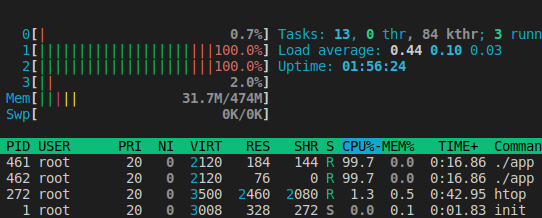
\includegraphics[width=0.7\textwidth]{imageSources/MultiCPU.png.png}
    \caption{Multi Core usage}
    \label{fig:MultiCore}
\end{figure}
\newpage
\subsection{Exercice 2}
Il a été observé que si l'on lance le programme et que l'on essaie de limiter le
nombre de bytes possibles alors qu'il a déjà atteint le quota, l'écriture est
bloquée et la limite ne peut être fixée. Cependant si l'on écrit la limite avant
que le programme ne l'ait atteinte, elle sera bien fixée et le programme
s'arrêtera lorsqu'il atteindra cette limite.\newline
Commande pour limiter la quantité max de mémoire :
\begin{minted}[linenos=false]{shell}
echo 20M > /sys/fs/cgroup/set/program/memory.limit_in_bytes
\end{minted}

Nous avons également pu observer que si l'on crée deux cgroup de limitation de
mémoire, un de 20M et l'autre de 30M. Si l'on ajoute notre PID dans celui de 20M
puis dans celui de 30M, au moment de l'ajout dans celui de 30M il est
automatiquement retiré des tasks du cgroup qui limitait à 20M.\newline

Nous avons créé un script pour limiter la mémoire et celui-ci se lance de la
manière suivante : 
\begin{minted}[linenos=false]{shell}
    ./set_memory_limit <PID> <MEMORY_LIMIT>
\end{minted}

\subsection{Exercice 3}


\chapter{TP 6}
\section{Résumé du laboratoire}

\section{Synthèse des connaissances acquises}
\subsection{Non acquis}

\subsection{Acquis, mais à exercer}

\subsection{Parfaitement acquis}

\section{Feedback}

\end{document}


